\documentclass[12pt,a4paper]{article}

\usepackage[T1]{fontenc}
\usepackage[utf8]{inputenc}
\usepackage[spanish,es-tabla,es-noshorthands]{babel}
\usepackage{lmodern}
\usepackage{microtype}
\usepackage[margin=2.1cm]{geometry}
\usepackage{amsmath}
\usepackage{graphicx}
\usepackage{booktabs}
\usepackage{array}
\usepackage{caption}
\usepackage{float}
\usepackage[hidelinks]{hyperref}

% Funciona compilando desde informe/ (repositorio) o subiendo figuras/ junto al .tex (Overleaf).
\graphicspath{{../figuras/}{figuras/}{./}}
\captionsetup{font=small,labelfont=bf}
\setlength{\parskip}{0.35em}
\setlength{\parindent}{0pt}

\title{\textbf{Taller 6: generación de texto con \emph{María}\\y traducción español--inglés con seq2seq}}
% Agregar aquí a los demás integrantes del grupo.
\author{Grupo 6 \\ Camilo García \\[0.3em]
  \small Procesamiento de Lenguaje Natural --- Maestría \\
  \small Código: \url{https://github.com/CamiloGarcia06/maestria-pln/tree/taller-6}}
\date{Octubre de 2026}

\begin{document}
\maketitle

\begin{abstract}
\noindent
Entrenamos dos tipos de modelos a partir del colab del curso (\emph{Deep Learning with Python}, 3.ª ed.).
En el punto~1, un modelo de lenguaje por caracteres con GRU aprende a escribir como \emph{María}
(Jorge Isaacs, 1867); con validación, \emph{early stopping} y dos capas más pequeñas, la perplejidad
baja de 5,41 (el colab) a 3,90. En el punto~2, con \emph{Combined Data es-ES} construimos 71.242
pares de oraciones y comparamos el GRU seq2seq del colab con un Transformer. Implementamos BLEU,
ROUGE y F1 desde cero: en prueba, el Transformer obtiene un BLEU de 28,7 contra 15,7 del GRU, con
menos de la mitad de parámetros, y su ventaja crece con el largo de la oración.
\end{abstract}

%======================================================================
\section{Punto 1: modelo de lenguaje por caracteres con \emph{María}}

\subsection{Datos y tokenización}

Descargamos los 65 capítulos de \emph{María} desde es.wikisource: 499 mil caracteres, 88 mil palabras
y 88 caracteres distintos. El token es el \textbf{carácter}: con palabras habría 11.947 tipos
distintos, muchos con una sola aparición en un libro tan corto. Usamos
\texttt{TextVectorization(split="character", standardize=None)} para conservar mayúsculas, tildes,
\texttt{¿¡} y la raya de diálogo. La validación es el \textbf{último 10\,\%} de la novela, separado por
posición para que ninguna ventana de validación se solape con una de entrenamiento.

Los dos hiperparámetros de la entrada cumplen papeles distintos:
\begin{itemize}\setlength{\itemsep}{0pt}
  \item \textbf{Tamaño del vocabulario = 90}: los 88 caracteres más el relleno (id 0) y \texttt{[UNK]} (id 1).
    Sale de los datos y fija el tamaño del \emph{Embedding} y de la capa de salida, es decir, los parámetros.
  \item \textbf{Longitud de la secuencia = 100}: cada ejemplo es una ventana de 100 caracteres y el objetivo
    es la misma ventana corrida un carácter. La elegimos nosotros y no cambia ningún parámetro, porque la
    GRU usa los mismos pesos en cada paso: cambia la forma del tensor y el contexto disponible.
\end{itemize}

\subsection{Arquitectura}

La Tabla~\ref{tab:arq-lm} muestra el mejor modelo (D), con la forma del tensor para un lote de 64 ventanas.
La GRU usa \texttt{return\_sequences=True} para producir una predicción en cada posición, de modo que cada
ventana aporta 100 ejemplos de entrenamiento. La pérdida es la entropía cruzada,
$-\log p(\text{carácter correcto})$, optimizada con Adam.

\begin{table}[H]
\centering\small
\begin{tabular}{llr}
\toprule
Capa & Forma de salida & Parámetros \\
\midrule
Entrada (ids de caracteres)            & (64, 100)      & --- \\
Embedding $90 \times 256$              & (64, 100, 256) & 23.040 \\
GRU 512 + Dropout 0,3                  & (64, 100, 512) & 1.182.720 \\
GRU 512 + Dropout 0,3                  & (64, 100, 512) & 1.575.936 \\
Dense 90 + softmax                     & (64, 100, 90)  & 46.170 \\
\midrule
\textbf{Total} & & \textbf{2.827.866} \\
\bottomrule
\end{tabular}
\caption{Arquitectura del modelo D. El del colab (A) tiene una sola GRU de 1024 y 4.053.594 parámetros.}
\label{tab:arq-lm}
\end{table}

\subsection{Experimentos}

Medimos la entropía cruzada por carácter en validación, también como perplejidad ($e^{\text{pérdida}}$)
y bits por carácter (Tabla~\ref{tab:exp-lm}).

\begin{table}[H]
\centering\small
\begin{tabular}{llrrr}
\toprule
Exp. & Cambio & Pérdida val. & Perplejidad & Exactitud \\
\midrule
A & Colab tal cual: 5 épocas, dropout 0,1                  & 1,688 & 5,41 & 49,2\,\% \\
B & A + hasta 40 épocas con \emph{early stopping}           & 1,397 & 4,04 & 57,8\,\% \\
C & B + ventanas solapadas (\texttt{paso=25}), dropout 0,3  & 1,390 & 4,02 & 57,7\,\% \\
D & C con 2 GRU de 512 (2,8\,M parámetros)                  & \textbf{1,361} & \textbf{3,90} & \textbf{58,4\,\%} \\
\bottomrule
\end{tabular}
\caption{Experimentos del modelo de lenguaje en validación.}
\label{tab:exp-lm}
\end{table}

\begin{figure}[H]
\centering
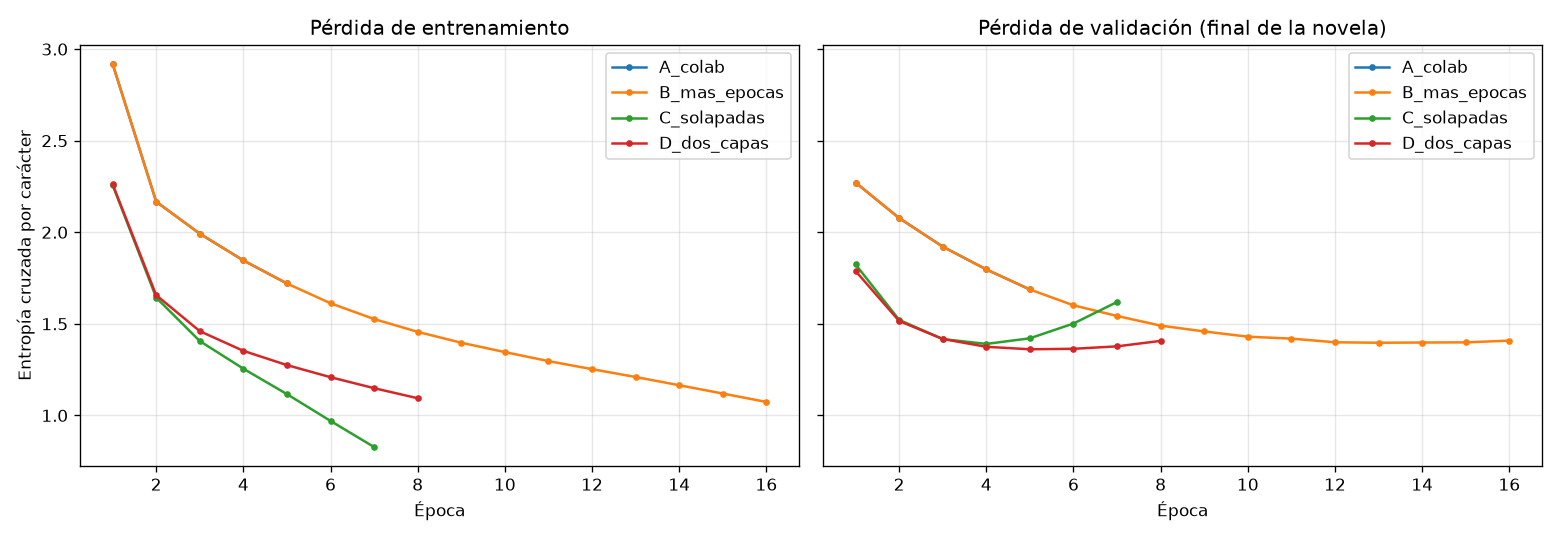
\includegraphics[width=0.82\linewidth]{01_curvas_lm.png}
\caption{Curvas de pérdida. En C, la pérdida de entrenamiento sigue bajando mientras la de validación sube desde la época~4.}
\label{fig:curvas}
\end{figure}

El colab entrena poco: solo con más épocas (B) la perplejidad baja de 5,4 a 4,0. Con un libro de
medio millón de caracteres y 4 millones de parámetros, el problema es el \textbf{sobreajuste}
(Figura~\ref{fig:curvas}); lo controlan el \emph{early stopping}, el dropout y un modelo más pequeño.
Las ventanas solapadas (C) solo aceleran la convergencia. El modelo D, con dos capas y menos parámetros,
generaliza mejor. Una pérdida de 1,361 equivale a asignar, en promedio, un 26\,\% de probabilidad al
carácter correcto entre 90, y una perplejidad de 3,9 a dudar entre unas cuatro opciones.

\subsection{Generación y temperatura}

Para generar, copiamos los pesos a un modelo paso a paso que recibe un carácter y el estado de la GRU,
y devuelve la distribución del siguiente carácter y el estado nuevo. El colab elige siempre el más probable
(\emph{greedy}) y cae en bucles («de la casa de la casa\ldots»). En su lugar muestreamos de
$\mathrm{softmax}(\log p / T)$ y elegimos $T$ midiendo 10 textos de 600 caracteres por temperatura
(Tabla~\ref{tab:temp}): palabras que existen en el libro, \emph{distinct-2} (bigramas distintos sobre totales)
y 5-gramas copiados de la novela.

\begin{table}[H]
\centering\small
\begin{tabular}{lrrr}
\toprule
Temperatura & Palabras válidas & Distinct-2 & 5-gramas copiados \\
\midrule
greedy & 100,0 & 4,0 & 0,8 \\
0,2 & 100,0 & 34,0 & 2,8 \\
\textbf{0,5} & \textbf{97,6} & \textbf{65,0} & \textbf{1,1} \\
0,8 & 89,9 & 84,7 & 0,1 \\
1,2 & 72,2 & 94,6 & 0,0 \\
\bottomrule
\end{tabular}
\caption{Calidad contra diversidad según la temperatura (en \%).}
\label{tab:temp}
\end{table}

$T=0{,}5$ equilibra ortografía y variedad sin recitar el libro. Con ella el modelo D escribe:

\begin{quote}\small\itshape
María y yo de comprender que la parte de mi madre, que ya no le perdiera yo que me entregó a mí.
---¿Y eso con el caballo no debe decir que es el momento de que se le había pasado por lo que había
precidido a Tránsito? ---le preguntó al fin. ---Sí ---le respondí.
\end{quote}

El estilo de la novela está presente: diálogos con raya, «le respondí», los personajes y el vocabulario
de la hacienda. Falta coherencia más allá de una frase, algo esperable con 100 caracteres de contexto.

%======================================================================
\section{Punto 2: traducción español $\rightarrow$ inglés}

\subsection{Datos}

\emph{Combined Data es-ES} contiene 53.043 publicaciones en inglés con su traducción automática al español.
Las publicaciones son largas (mediana de 53 palabras), así que las partimos en oraciones y emparejamos la
$i$-ésima con la $i$-ésima cuando ambos idiomas tienen el mismo número de oraciones. Tras filtrar (de 2 a 20
palabras, razón de largos entre 0,5 y 2, sin \emph{mojibake}, traducidas y sin duplicados) quedan
\textbf{71.242 pares}, 4,6 veces más que usando solo publicaciones cortas. Dividimos 80/10/10
\textbf{por publicación} y retiramos de validación y prueba 446 oraciones repetidas de entrenamiento, para
medir traducción y no memoria: 57.257 / 6.747 / 6.792 pares.

Aquí el token es la \textbf{palabra}. Cada idioma tiene su vocabulario, limitado a las \textbf{15.000}
palabras más frecuentes (el resto es \texttt{[UNK]}, el 2,8\,\% de los tokens en inglés de validación), y la
longitud es de \textbf{20} tokens, con relleno o corte. El inglés se envuelve en \texttt{[start]}\ldots\texttt{[end]}
y se tokeniza con 21: los primeros 20 tokens son la entrada del decodificador y los últimos 20 el objetivo
(\emph{teacher forcing}).

\subsection{Arquitecturas}

\textbf{GRU seq2seq (colab).} El codificador lee el español con una GRU \textbf{bidireccional} de 1024 cuyas dos
direcciones se suman en un único vector, (64, 1024). Ese vector es el estado inicial de la GRU del
decodificador, que produce (64, 20, 1024) y, tras una Dense con softmax, (64, 20, 15000). Toda la oración
debe caber en ese vector: es el \textbf{cuello de botella}. Tiene 34,9\,M parámetros, 15,4\,M de ellos en la
capa de salida.

\textbf{Transformer} \cite{vaswani}. Construido con \texttt{keras\_hub}: embeddings de token y de posición
de 256 (la atención no ve el orden), un \texttt{TransformerEncoder} y un \texttt{TransformerDecoder}
con 8 cabezas de 32 dimensiones y capa interna de 2.048. El codificador entrega un vector por palabra,
(64, 20, 256), y el decodificador consulta todas las palabras del español en cada paso mediante atención cruzada:
\[
\mathrm{Atención}(Q,K,V) = \mathrm{softmax}\!\left(\frac{QK^{\top}}{\sqrt{d}}\right)V .
\]
Su autoatención usa una máscara causal para no mirar palabras futuras. Tiene 14,4\,M parámetros.

Ambos se entrenan con Adam y \emph{early stopping}, y traducen con decodificación \emph{greedy} desde
\texttt{[start]} hasta \texttt{[end]}. El Transformer entrena en 130\,s contra 533\,s del GRU, porque procesa
las 20 posiciones en paralelo. Su exactitud por token en validación es de 58,5\,\% contra 48,6\,\%.
La \texttt{val\_loss} de Keras no es comparable entre ambos: el Transformer propaga la máscara de relleno y
promedia sobre los tokens reales, mientras el GRU promedia sobre las 20 posiciones. Medida por token real,
la entropía cruzada es 2,44 para el Transformer y 2,99 para el GRU.

\subsection{Métricas}

Las tres métricas están implementadas en \texttt{metricas.py} sobre texto normalizado.
\textbf{BLEU} \cite{bleu} es la media geométrica de las precisiones de $n$-gramas $p_n$ ($n=1..4$) con conteo
recortado, multiplicada por una penalización por brevedad:
$\mathrm{BLEU}=\min\!\left(1,e^{1-r/c}\right)\exp\!\big(\tfrac14\sum_{n}\log p_n\big)$.
\textbf{ROUGE-1/2} \cite{rouge} es la medida F del traslape de unigramas o bigramas, y \textbf{ROUGE-L}
la de la subsecuencia común más larga. El \textbf{F1 de tokens} es la media armónica de precisión y
\emph{recall} sobre la bolsa de palabras. Nuestras implementaciones coinciden con \texttt{sacrebleu} y
\texttt{rouge-score} hasta el tercer decimal (BLEU de validación 16,122 en ambos). El F1 de tokens resulta
\textbf{idéntico} a ROUGE-1: los dos son la medida F de la intersección recortada de unigramas. Lo
informativo es contrastar F1, que ignora el orden, con BLEU y ROUGE-2, que lo exigen.

\subsection{Resultados}

\begin{table}[H]
\centering\small
\begin{tabular}{lrrrrr}
\toprule
Modelo & BLEU & ROUGE-1 & ROUGE-2 & ROUGE-L & F1 \\
\midrule
Copiar el español (línea base) & 0,6 & 4,3 & 0,7 & 4,3 & 4,3 \\
GRU seq2seq (colab)            & 15,7 & 45,1 & 22,8 & 43,0 & 45,1 \\
\textbf{Transformer}           & \textbf{28,7} & \textbf{58,2} & \textbf{35,6} & \textbf{56,4} & \textbf{58,2} \\
\bottomrule
\end{tabular}
\caption{Resultados en el conjunto de prueba (6.792 oraciones, usado una sola vez).}
\label{tab:test}
\end{table}

El Transformer casi duplica el BLEU del GRU y le saca unos 13 puntos en el resto de métricas
(Tabla~\ref{tab:test}). La brecha relativa es mayor en las métricas de orden: el GRU acierta el 45\,\% de
las palabras, pero pocas secuencias. La Figura~\ref{fig:largo} confirma el cuello de botella: de 2--5 a
16--20 palabras, el BLEU del GRU cae a un tercio (28,6 $\rightarrow$ 9,5), mientras el del Transformer
pierde un 37\,\% (37,5 $\rightarrow$ 23,6).

\begin{figure}[H]
\centering
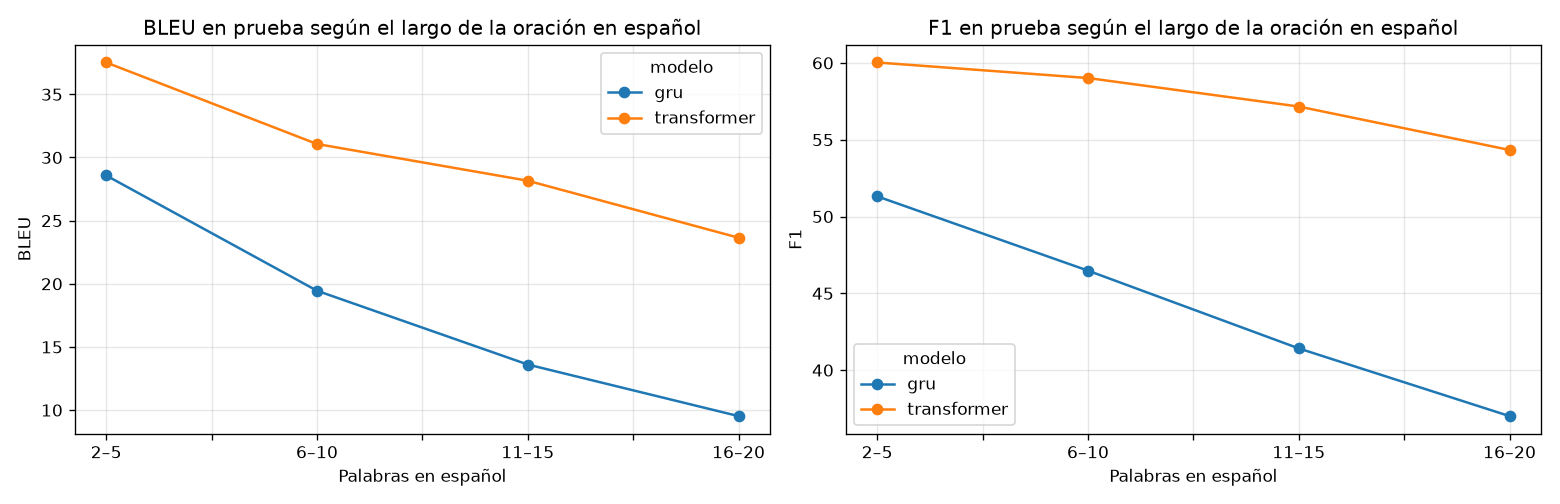
\includegraphics[width=0.9\linewidth]{06_por_largo.png}
\caption{BLEU y F1 en prueba según el número de palabras de la oración en español.}
\label{fig:largo}
\end{figure}

\begin{table}[H]
\centering\small
\begin{tabular}{>{\raggedright\arraybackslash}p{4.6cm}>{\raggedright\arraybackslash}p{5.2cm}>{\raggedright\arraybackslash}p{5.2cm}}
\toprule
Español & GRU & Transformer \\
\midrule
Hoy es mi último día. & today is my last day & today is my last day \\
Y será como si nunca hubiera existido, como si nunca hubiera experimentado nada de esto.
  & and it will always be like if i never had it ever would have done with this
  & and it will be like i have never existed like i never experienced anything \\
Muy buen ambiente escuchando a Raki cantar esta canción
  & very busy story [UNK] [UNK] [UNK] this morning
  & very good link to [UNK] sing this song \\
\bottomrule
\end{tabular}
\caption{Traducciones de prueba. El GRU suena fluido pero pierde el contenido; los nombres raros quedan como [UNK].}
\label{tab:ejemplos}
\end{table}

%======================================================================
\section{Conclusiones}

\begin{enumerate}\setlength{\itemsep}{0pt}
  \item Un GRU por caracteres entrenado solo con \emph{María} aprende ortografía, puntuación de diálogo y
    personajes. Con un libro pequeño el problema es el sobreajuste: la perplejidad baja de 5,4 a 3,9 con
    validación, \emph{early stopping} y un modelo con menos parámetros.
  \item La decodificación importa tanto como el modelo: \emph{greedy} se repite, y $T=0{,}5$ equilibra
    97,6\,\% de palabras reales con 65\,\% de bigramas distintos.
  \item Partir las publicaciones en oraciones alineadas multiplicó por 4,6 los datos de traducción.
  \item El Transformer supera al GRU seq2seq en todas las métricas (BLEU 28,7 contra 15,7) con 14,4\,M
    parámetros frente a 34,9\,M y en un cuarto del tiempo, y su ventaja crece con la longitud de la oración.
  \item F1 de tokens y ROUGE-1 son la misma medida; la comparación útil es entre métricas con y sin orden.
\end{enumerate}

\textbf{Limitaciones.} El español del corpus es traducción automática, así que el modelo aprende a invertir
ese traductor con su ruido; hay una sola referencia por oración; el vocabulario cerrado produce \texttt{[UNK]}
(las subpalabras o un modelo preentrenado lo resolverían), y cada configuración se corrió con una sola semilla.

\begin{thebibliography}{9}\small
\bibitem{chollet} F. Chollet y M. Watson. \emph{Deep Learning with Python}, 3.ª ed. Manning, 2025.
\bibitem{vaswani} A. Vaswani et al. Attention is all you need. \emph{NeurIPS}, 2017.
\bibitem{bleu} K. Papineni, S. Roukos, T. Ward y W.-J. Zhu. BLEU: a method for automatic evaluation of machine translation. \emph{ACL}, 2002.
\bibitem{rouge} C.-Y. Lin. ROUGE: a package for automatic evaluation of summaries. \emph{ACL Workshop}, 2004.
\bibitem{gru} K. Cho et al. Learning phrase representations using RNN encoder--decoder for statistical machine translation. \emph{EMNLP}, 2014.
\bibitem{distinct} J. Li et al. A diversity-promoting objective function for neural conversation models. \emph{NAACL}, 2016.
\end{thebibliography}

\end{document}
